%% ----------------------------------------------------------------
%% synopsis.tex -- MAIN FILE (the one that you compile with LaTeX)
%% ---------------------------------------------------------------- 

% Set up the document
\documentclass[a4paper, 12pt, twoside]{synopsis}  % Use the "synopsis" style, based on the ECS synopsis style by Steve Gunn
\graphicspath{{Figures/}}  % Location of the graphics files (set up for graphics to be in PDF format)

% Include any extra LaTeX packages required
\usepackage[square, numbers, comma, sort&compress]{natbib}  % Use the "Natbib" style for the references in the Bibliography
\usepackage{verbatim}  % Needed for the "comment" environment to make LaTeX comments
\usepackage{missing_packages/vector}  % Allows "\bvec{}" and "\buvec{}" for "blackboard" style bold vectors in maths
\usepackage{textcomp}
\usepackage{tikz}
\usepackage{setspace} 
\hypersetup{urlcolor=black, colorlinks=true}  % Colours hyperlinks in blue, but this can be distracting if there are many links.
\usepackage{times}
%\usepackage{missing_packages/lineno}
%\linenumbers
%% ----------------------------------------------------------------
\begin{document}
%\frontmatter	  % Begin Roman style (i, ii, iii, iv...) page numbering
% Set up the Title Page
\title  {Multi Segmented Image Transfer in Delay Tolerant Networks using Bandwidth Reduction Technique}
\authors  {\texorpdfstring
            {\href{pratyush.anand@st.com
}
            {Pratyush Anand}}
            {Pratyush Anand}
            }
\addresses  {\groupname\\\deptname\\\univname}  % Do not change this here, instead these must be set in the "synopsis.cls" file, please look through it instead
\date       {\today}
\subject    {}
\keywords   {}

\maketitle

%% ----------------------------------------------------------------

\setstretch{1.0}  % It is better to have smaller font and larger line spacing than the other way round

\pagestyle{plain}  % Return the page headers back to the "fancy" style


%% ----------------------------------------------------------------

\section{Introduction}
\indent Surveillance systems are ubiquitous and find many applications
in areas such as traffic monitoring, elderly care etc. Therefore, there
is a pressing need to evolve methods for conserving bandwidth while the
video data is transported from the point of acquisition to the point of
observation. Moreover, an increasing number of video sources rely on
resource constrained (bandwidth-limited, delay-tolerant) networks such
as Zigbee, DASH7 specially in smart home applications for the video
transport. With such networks at layer 1 and 2, there is tremendous need
to conserve/preserve the bandwidth needed by each video stream / all
video streams collectively. We propose a method by which a few
pre-processing operations allow us to still carry out the primary
objective – surveillance – while achieving large and impressive savings
on the required bandwidth.\\
\indent Video surveillance system can be integrated with existing home
network, but it is very important to achieve reduction in amount of
data to be transmitted due to lack of end to end connectivity. A low
data rate node also allows the system to remain in sleep mode for longer
durations and hence prolongs longer battery life.\\
\indent For surveillance data, only a few segments of image need to be
transmitted (the fast changing scenes).  Transmitting only significant
features pre-extracted locally from the image can reduce transmission
requirement significantly. However, this minimization of content must
allow reconstruction of the image with relevant details at the other
end. By extracting semantic information from deduced features, we reduce
the data rate even further. \\
\indent Automatic scene analysis, followed by extraction of desired
information can be complex, especially when application is targeted for
outdoor monitoring.  Sometime background of the scene can be fast
changing, while in some other scene ambient light can be different.
Similarly, there can be many other hurdles in the process of automation.
But if an efficient background detection algorithm is chosen then, these
issues can be addressed. Further, the selected algorithm must allow
information extraction almost in real time. With latest research in
computer vision ~\cite{3} ~\cite{5}, it seems that such a task could be
viable with low cost embedded system.\\
\indent Surveillance camera is normally kept at some distance from the
object. Therefore motion based descriptor is a good candidate for true
object detection.\\
\section{Objective}
\indent	In this work we propose a solution for efficiently transforming
video data   over   a delay   tolerant   network.  We have addressed
following problem in this work.\\
\begin{enumerate}
\item Evaluation of background subtraction algorithms (with reasonably
good result for surveillance applications) in terms of computational
complexities. 
\item Evaluation of different techniques of moving object
skeletonization in terms of its suitability to calculate motion
descriptor feature. 
\item Development of low computation algorithm to detect objects using
motion descriptor.
\item Integration of proposed algorithm with low cost COTS embedded
environment.
\end{enumerate}
\section{Implementation}
\indent We have selected Vibe ~\cite{5} algorithm by Barnich and Van
Droogenbroeck for background subtraction, as it comes out to be
computationally most efficient. Since authors have not provided C code,
so we have developed our own C code for this algorithm.\\
\indent Since surveillance object might be distant, so We have selected
skeleton motion approach for human detection. We have evaluated
different skeletonization method and finally star skeletonization method
has been used. Star skeletonization approach provides a easy way for leg
motion analysis. Analysis of leg motion allows us to detect human from
human, vehicle and animal. Since we have used \textbf{S}keleton
\textbf{M}otion \textbf{A}nalyzer for object detection, therefore we
name our implementation as SMA.\\
\section {Result Summary}
\indent We observe that with SMA, we are able to detect a moving person
after a movement of 3 steps. Fig.  \ref{pipeline_images} shows output
images at different stages of the implementation.\\
\indent We have also done experiments with negative images like a person
moving on bicycle, or a vehicle moving on road. SMA is successfully able
to discriminate between these objects. Fig. \ref{negative_inputs} shows
how it rejects moving vehicle and bicycle and  does not detect them as
human.\\
\begin{figure}[!h]
\centering
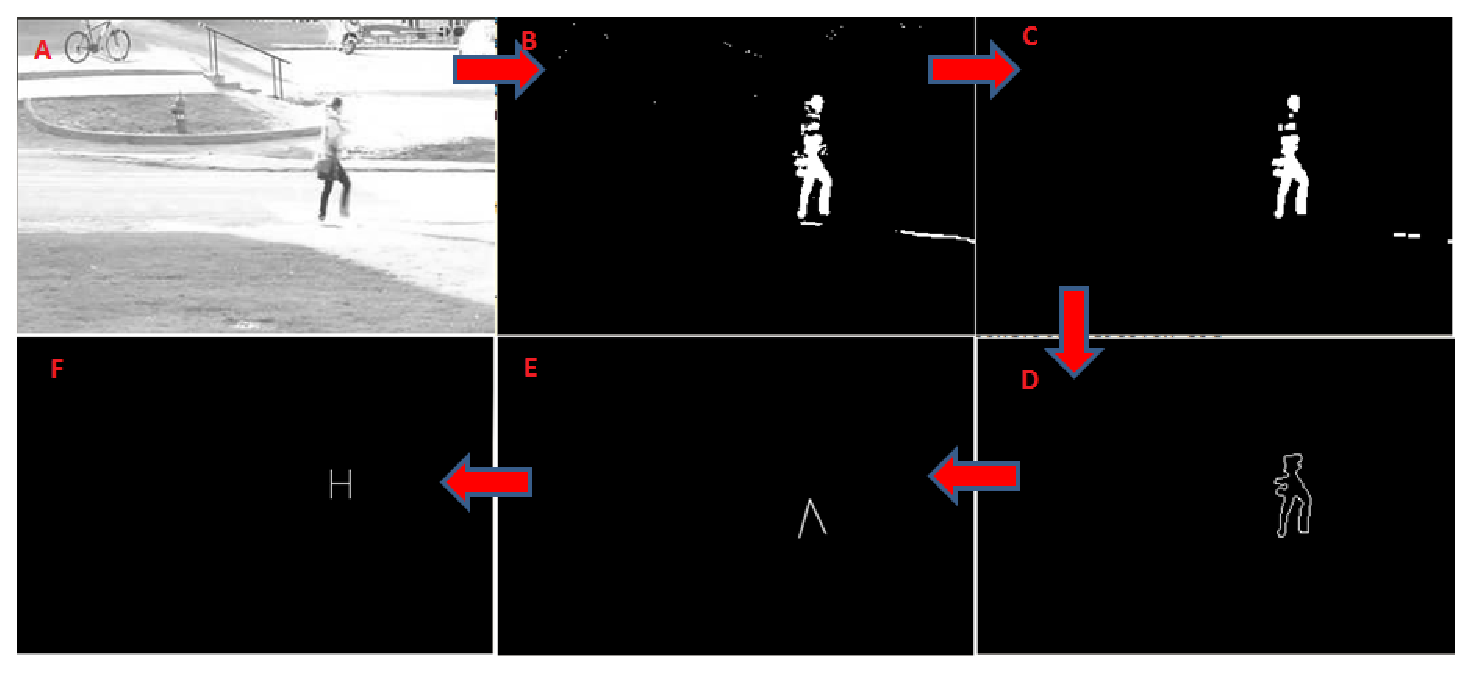
\includegraphics[scale=0.30]{Figures/pipeline_images}
\caption{Images at different stages of processing. (From top left in
clockwise order) \textbf{(a.)} Gray Scale input frame
\textbf({b.)}Foreground extracted image using Vibe \textbf{(c.)} Cleaned
image \textbf{(d.)} Contour of moving object \textbf{(e.)} Plot of three points
of interest, centroid and two distance peaks nearer to bottom left and
bottom right corner of bounding box \textbf{(f.)} Virtual representation
of scene} 
\label{pipeline_images}
\end{figure}
\begin{figure}[!h]
\centering
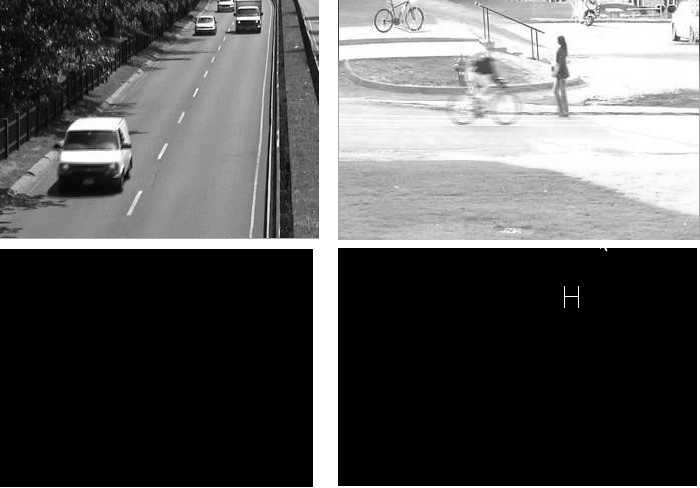
\includegraphics[scale=0.30]{Figures/negative_inputs}
\caption{Input and output in case of negative images}
\label{negative_inputs}
\end{figure}
\indent We have implemented and executed SMA, HAAR ~\cite{2} and
covariance ~\cite{14} feature based detection algorithm on both x86
desktop computer and embedded ARM platform. Comparison of execution time
has been shown in Fig.  \ref{pipeline_execution_time}. It shows a
definite improvement in execution speed of SMA over HAAR and covariance
feature based approach.  SMA takes just 3.6 ms on the average, while
HAAR and covariance feature based algorithm take around 20 ms and 248 ms
respectively per frame at x86 platform having DMIPS = 800. Comparison of
timing at ARM platform with DMIPS = 44 shows that SMA takes 182 ms
on the average, while HAAR and covariance feature based algorithm take
around 942 ms and 4.65 s respectively per frame.  \\
\begin{figure}[!h]
\centering
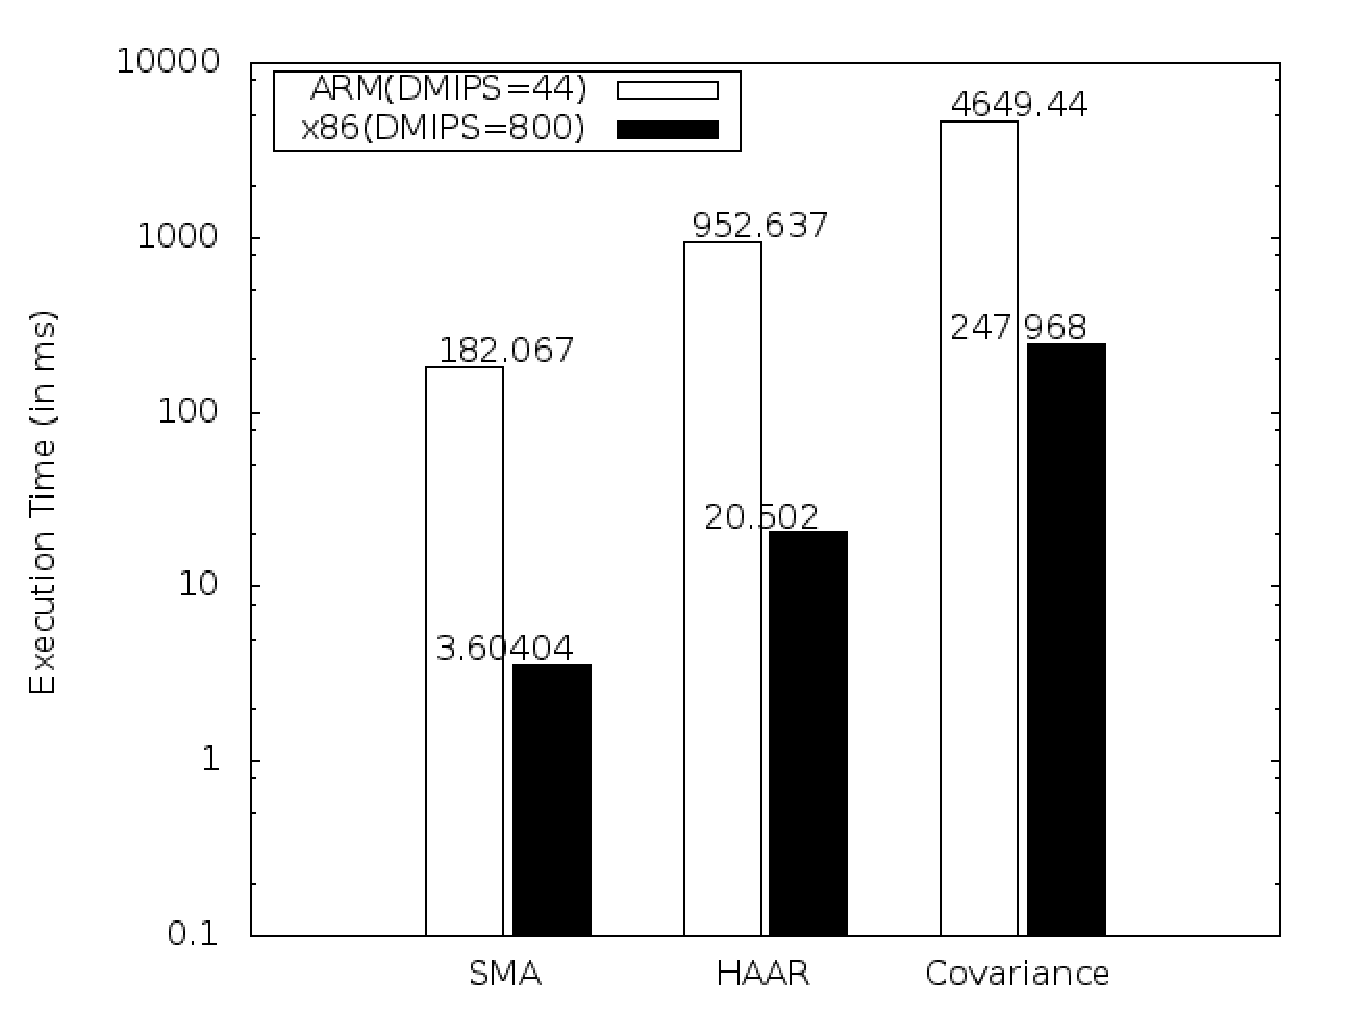
\includegraphics[scale=0.30]{Figures/pipeline_execution_time}
\caption{Execution time of evaluated algorithms with a ARM and x86
platform}
\label{pipeline_execution_time}
\end{figure}
\section {Publications}
\indent A paper titled ``Image Analysis for Ultra Low Bandwidth Video
Surveillance System`` is under communication.\\
%% ----------------------------------------------------------------

\label{Bibliography}
\addtotoc{Bibliography}
\lhead{\emph{Bibliography}}  % Change the left side page header to "Bibliography"
%\bibliographystyle{ieeetr}  % Use the "unsrtnat" BibTeX style for formatting the Bibliography
\bibliographystyle{apalike}
\bibliography{Bibliography}  % The references (bibliography) information are stored in the file named "Bibliography.bib"
\cleardoublepage


\end{document}  % The End
%% ----------------------------------------------------------------
